\documentclass[12pt]{article}

\usepackage[utf8]{inputenc}
\usepackage[english, russian]{babel}

% "А вот теперь --- слайды!"
\usepackage{slides}

% ШРИФТЫ
% Нужны рубленные шрифты -- раскомментируйте стоку ниже.
% Нужны шрифты с засечками --- закомментируйте эту строку.
% \renewcommand{\familydefault}{\sfdefault} % Переключает на рубленный шрифт.
% Шрифты Times и Arial, если стоит пакет cyrtimes.
\IfFileExists{cyrtimes.sty}
    {
        \usepackage{cyrtimespatched}
    }
    {
        % А если Times нету, то будет CM...
    }

% \renewcommand{\seriesdefault}{b} % для шрифта с засечками, это предпочтительно
% \renewcommand{\seriesdefault}{sbc} % для рубленного шрифта


% Прочие пакетики
% Графика.
\usepackage{graphicx}

% Настройка презентации
% Студент и руководитель.
\def\Student{Миникс Игорь Владимирович}
\def\Advisor{Степанов Валерий Павлович}
% \def\Person
% \def\Affilation
% Титул
\def\Title{Разработка системы имитационного моделирования в форме библиотеки языка Haskell}
% Титул для нижнего колонтитула. Может быть сокращённым
\def\FooterTitle{\Title}
\def\SubTitle{Квалификационная работа}
\newcommand{\TitleSlide}{
    \addcontentsline{toc}{section}{\Title}%
    ~\vspace{1cm}

    \begin{center}
    {\huge \begin{spacing}{1}\Title\end{spacing}}

    {\SubTitle}
    \vspace{2cm}

    \ifthenelse{\isundefined{\Student}}{}
        {\small Студент: \Student\\}
    \ifthenelse{\isundefined{\Advisor}}{}
        {\small Руководитель: \Advisor\\}
    \ifthenelse{\isundefined{\Person}}{}
        {\Person\\}
    \ifthenelse{\isundefined{\Affilation}}{}
        {\Affilation\\}
    \end{center}
    \thispagestyle{empty}
}


% Верхний заголовок: пустой
% Нижний заголовок по-умолчанию:
% \lfoot{\Title} % слева
% \cfoot{} % цент пуст
% \rfoot{\thepage} % справа

% \renewcommand{\baselinestretch}{1.5}
% \linespread{1.6}


%% Переносы в презентации смотряся не очень.
\hyphenpenalty 10000
\sloppy


\begin{document}

% \raggedright -- грубое выавнивание по левому краю.
% \raggedright

\TitleSlide

% Команды section и subsection начинают новый слайд.

\section{Цель и задачи работы}
\small
\emph{Целью работы} является создание системы имитационного
моделирования, основанной на принципах и синтаксисе GPSS, позволяющей разрабатывать модели как часть более крупной программы на языке Haskell.

\subsubsection{Решаемые задачи}
\begin{enumerate}
\item Разработать синтаксис описания моделей схожий с синтаксисом
GPSS, но согласующийся с синтаксисом Haskell.
\item Выбрать подмножество блоков GPSS, которые следует реализовать
в системе.
\item Реализовать алгоритмы описания моделей и имитационного моделирования.
\item Провести тестирование разработанного программного обеспечения.
\end{enumerate}

\normalsize
%\section{Объекты GPSS}
%\begin{enumerate}
%\item Транзакты.
%\item Блоки.
%\item Устройства.
%\item Хранилища (памяти).
%\item Очереди.
%\item Ключи.
%\item Таблицы.
%\item И др.
%\end{enumerate}

%\section{Атрибуты транзактов}
%\begin{enumerate}
%\item Параметры.
%\item Приоритет.
%\item Текущий  блок.
%\item Следующий блок.
%\item Состояние.
%\end{enumerate}


%\section{Диаграмма состояний транзакта}

%\begin{center}
%\includegraphics[height=0.87\textheight]{inc/dia/transactionState}
%\end{center}%

%\section{Управление процессом моделирования в GPSS}

%\begin{center}
%\includegraphics[height=0.8\textheight]{inc/dia/gpss}
%\end{center}

\section{Пример моделируемой системы}

\includegraphics[width=\textwidth]{inc/dia/main}


\section{Подмножество реализуемых блоков}

\begin{enumerate}
\item GENERATE, TERMINATE~--- создание и уничтожение заявок.
\item ADVANCE~--- задержка продвижения транзактов
\item SEIZE, RELEASE~--- занятие и освобождение устройств.
\item ENTER, LEAVE~--- занятие и освобождение хранилищ.
\item PREEMPT, RETURN~--- занятие и освобождение устройств с абсолютным приоритетом.
\item TRANSFER~--- изменение порядка следования транзактов.
\end{enumerate}

\section{Опиcание модели как вычисление с состоянием}

\includegraphics[width=\textwidth]{inc/dia/StateIDEF}

\section{Синтаксис описания моделей}

\begin{minipage}[m]{.49\textwidth}
\centerline{GPSS}

\begin{verbatim}


GENERATE 10,2
QUEUE WaitingLine
SEIZE Worker
DEPART WaitingLine
ADVANCE 3
RELEASE Worker
TERMINATE 1

\end{verbatim}


\end{minipage}
%
\begin{minipage}[m]{.49\textwidth}
\vspace{1cm}
\centerline{HASKELL}

\begin{verbatim}

model = 
    do generate (10,2)
       queue "WaitingLine"
       seize "Worker"
       depart "WaitingLine"
       advance 3
       release "Worker"
       terminate 1

\end{verbatim}

\end{minipage}


\section{Состояние системы в процессе моделирования}

\includegraphics[width=\textwidth]{inc/dia/umlSim}


\section{Алгоритм имитационного моделирования}
%\begin{figure}
\centering
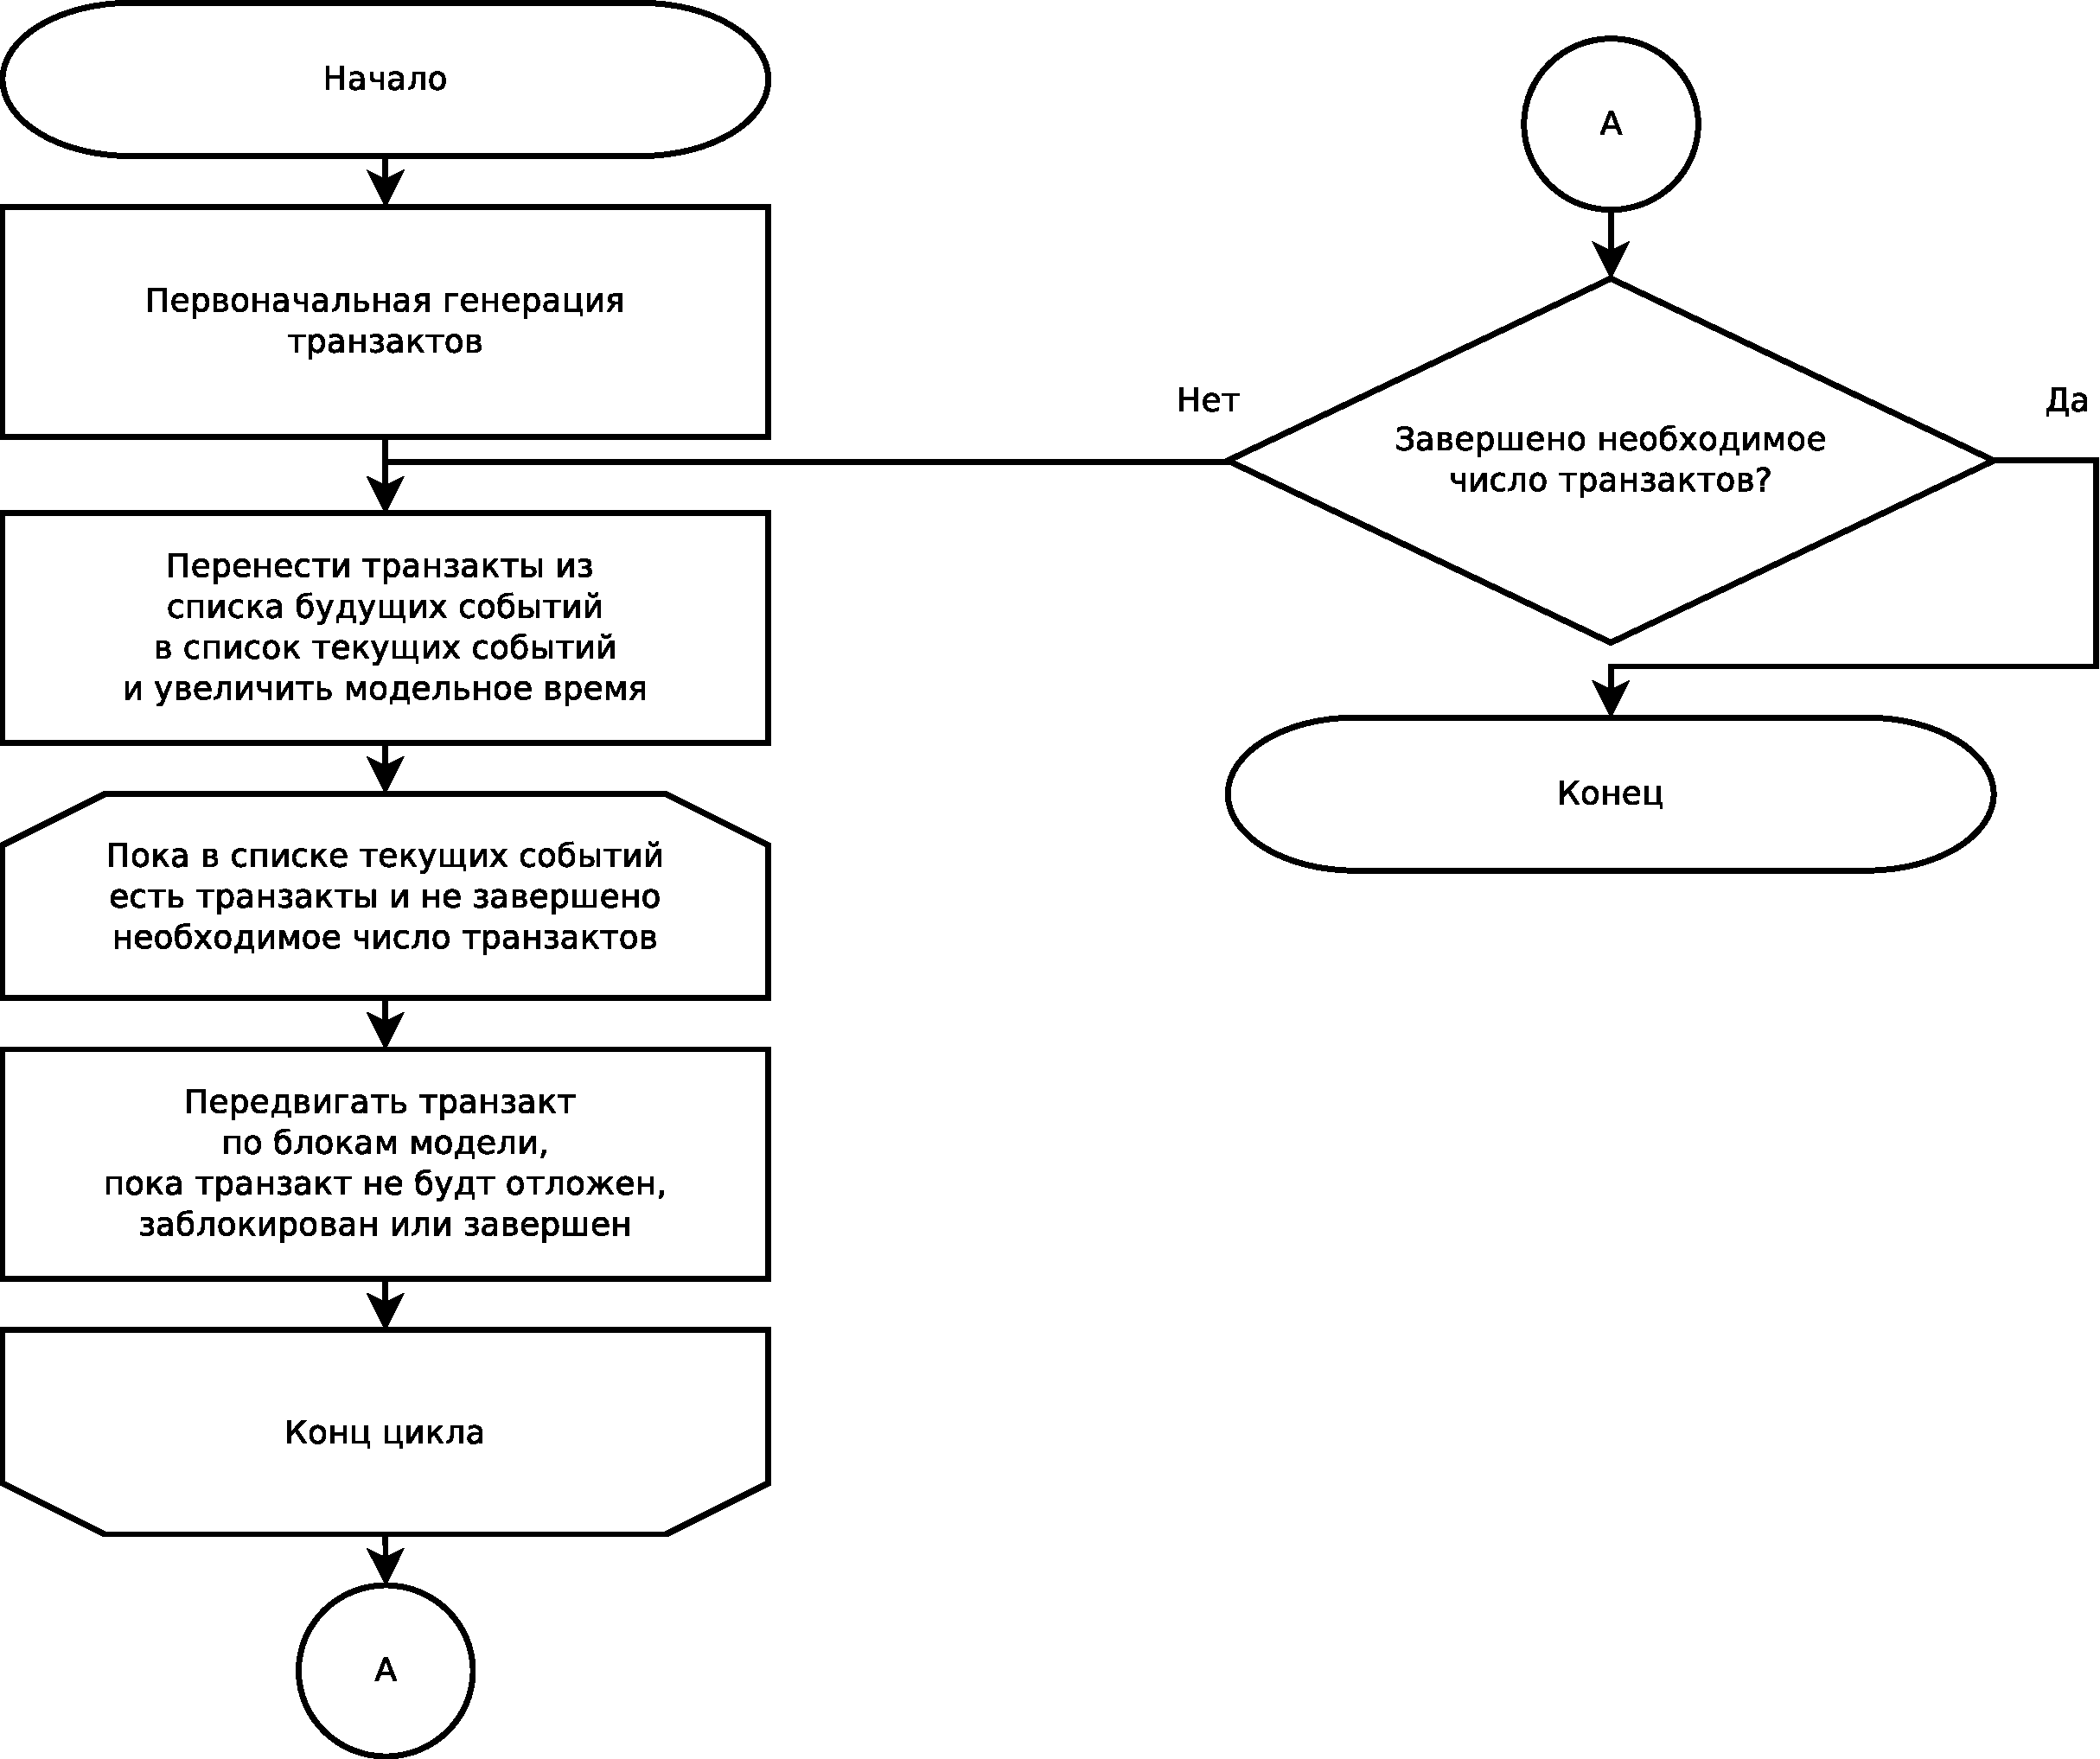
\includegraphics[height=0.75\textheight]{inc/dia/simFlowchartPres}
%\end{figure}

\section{Алгоритм продвижения транзактов}
\begin{minipage}[m]{.49\textwidth}
\includegraphics[width=\textwidth]{inc/dia/enterFlowchart}
\end{minipage}
\begin{minipage}[m]{.49\textwidth}
\includegraphics[width=\textwidth]{inc/dia/leaveFlowchart}
\end{minipage}


\section{Структура библиотеки}
\includegraphics[height=0.75\textheight]{inc/dia/libStructHuge}


\section{Алгоритм аналитического решения}
\vfill
\includegraphics[width=\textwidth]{inc/dia/idefAnalit}
\vfill

\section{Структура демонстрационной программы}
\includegraphics[height=0.75\textheight]{inc/dia/demoStruct}

%\section{Сравнение аналитической и имитационной модели}


%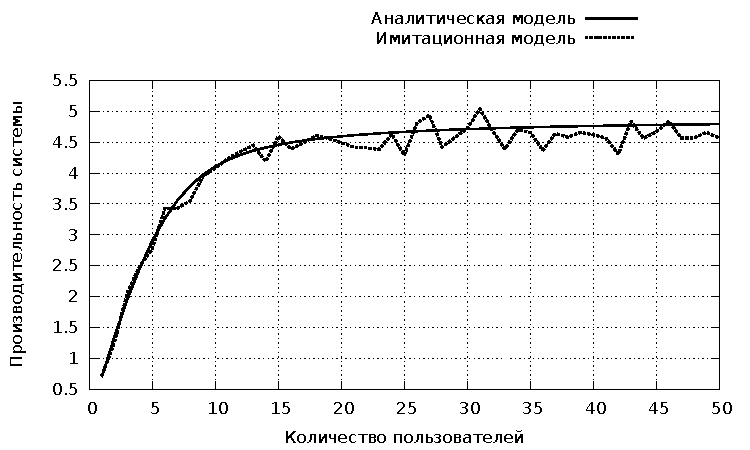
\includegraphics[height=0.75\textheight]{inc/pdf/plot1}

%\section{Сравнение аналитической и имитационной модели}
%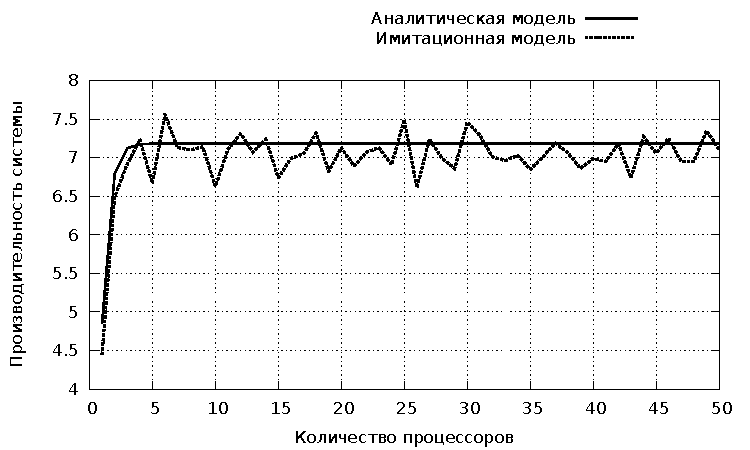
\includegraphics[height=0.75\textheight]{inc/pdf/plot2}

\section{Сравнение аналитической и имитационной модели}
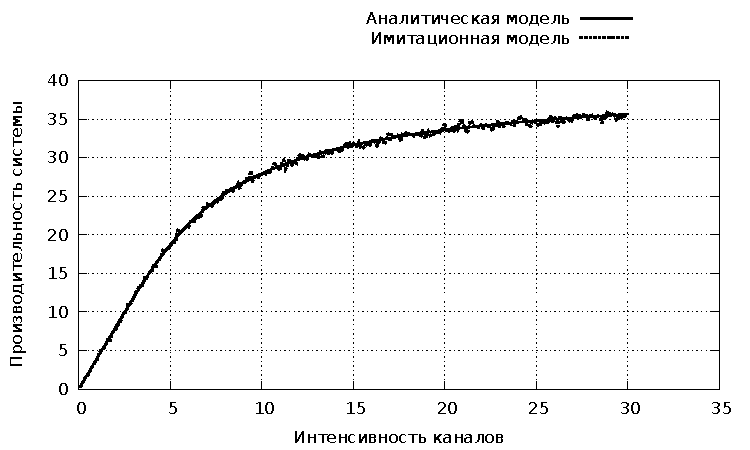
\includegraphics[height=0.75\textheight]{inc/pdf/plot3}

\section{Сравнение аналитической и имитационной модели}
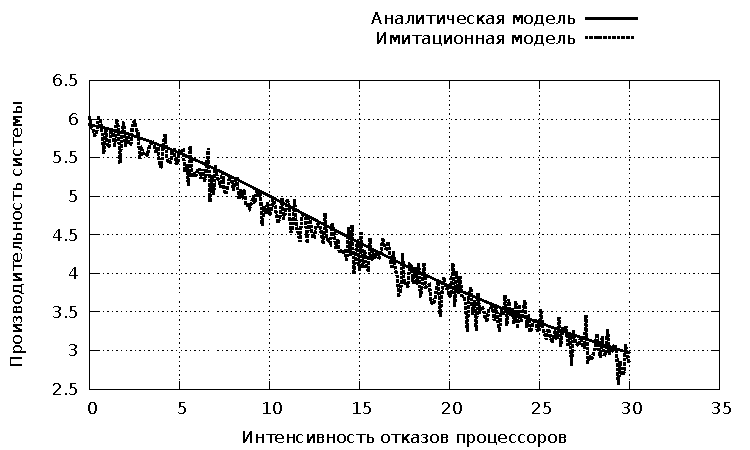
\includegraphics[height=0.75\textheight]{inc/pdf/plot4}

%\section{Сравнение аналитической и имитационной модели}
%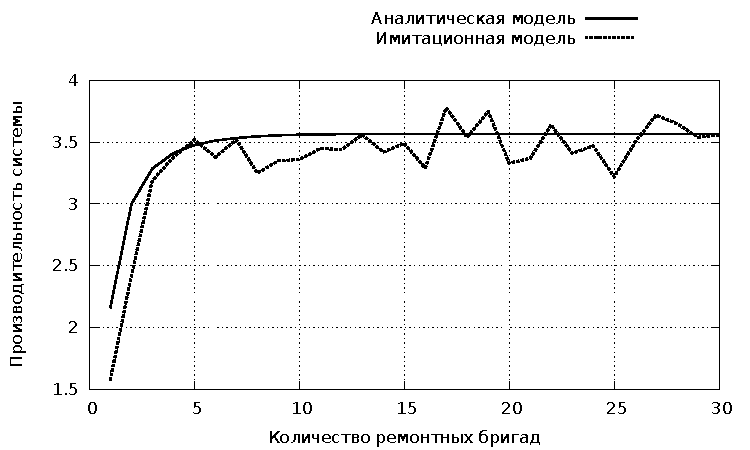
\includegraphics[height=0.75\textheight]{inc/pdf/plot5}


\section{Выводы}

\small

\begin{itemize}

\item В ходе работы была разработана и реализована бибилиотека имитационного моделирования, позволяющая описывать и исследовать заданный класс систем массового обслуживания.

\item Построены аналитическая и имитационная модель тестовой системы.

\item Реализована демонстрационная программа, показывающая возможности разработанной библиотеки.

\item Проведен ряд опытов, подтверждающих корректность разработанных алгоритмов и их реализации.

\end{itemize}
\normalsize
\end{document}
